\section{Teórico}

  \definicion{Topic:} Charge densities and potentials. Systems in 0-1-2-3D. Metals vs. insulators. Non-magnetic vs. magnetic systems.

  \definicion{Speaker:} Paolo GIANNOZZI (University of Udine, Italy)

\subsection{DFT}

  Dada una función unidimensional $L$-periódica $f$, la transformada de Fourier (FT) nos permite establecer que
    $$f(x) = \sum_n \tilde{f} (q_n) e^{iq_n x} \quad ; \quad \tilde{f} (q_n) = \frac{1}{L} \int f(x) e^{-iq_n x} dx$$

  donde
    $$q_n = n \frac{2\pi}{L} \quad ; \quad n \in \mathbb{Z}$$

  En el caso de la transformada de Fourier discreta (DFT) se considera un conjunto finito de valores, tanto para $q$ como para $x$, volviéndose ambas variables periódicas: los valores negativos son mapeados al correspondiente positivo.
    $$f(x) \rightarrow f_m \equiv f(x_m) \quad ; \quad x_m = m \frac{L}{N} \quad ; \quad m \in [0, N-1]$$
    $$\tilde{f}(q) \rightarrow \tilde{f}_n \equiv \tilde{f}(q_n) \quad ; \quad q_n = n \frac{2\pi}{L} \quad ; \quad n \in [0, N-1]$$

  El valor de $N$ tiene que ser lo suficientemente grande como para incluir correctamente todas las componentes de Fourier en el $q$-espacio.

  Reuniendo todo esto, la DFT se escribe como
    $$f_m = \sum_{n=0}^{N-1} \tilde{f}_n e^{i2\pi \frac{nm}{N}} \quad ; \quad x\text{-espacio}
    \quad\quad\quad\quad
    \tilde{f}_n = \sum_{m=0}^{N-1} f_m e^{-i2\pi \frac{nm}{N}} \quad ; \quad q\text{-espacio}$$

  Para extender esto a 3 dimensiones, consideramos primero un conjunto de vectores de la red recíproca $\vec{G}$ centrados en el origen, dados por
    $$\vec{G} = n_1^{'} \vec{G}_1 + n_2^{'} \vec{G}_2 + n_3^{'} \vec{G}_3$$

  siendo $\vec{G}_{1,2,3}$ los vectores primitivos. La grilla sobre el $G$-espacio es periódica por construcción. Análogamente en el $R$-espacio se tiene que
    $$\vec{r} = \frac{m_1}{N_1} \vec{R}_1 + \frac{m_2}{N_2} \vec{R}_2 + \frac{m_3}{N_3} \vec{R}_3 \quad ; \quad m_s\in[0, N_s - 1]$$

  siendo $\vec{R}_{1,2,3}$ los generadores de la red de Bravais. En el caso 3D también debemos tomar un conjunto finito. Para ello
    $$f(\vec{r}) = \sum_G \tilde{f} (\vec{G}) e^{i \vec{G}\cdot\vec{r}} \rightarrow f(m_1, m_2, m_3)
    \quad\quad\quad\quad
    \tilde{f}(\vec{G}) = \frac{1}{\Omega} \int f (\vec{r}) e^{-i \vec{G}\cdot\vec{r}} d \vec{r} \rightarrow \tilde{f}(n_1, n_2, n_3)$$
    $$f(m_1, m_2, m_3) = \sum_{n_1, n_2, n_3} \tilde{f} (n_1, n_2, n_3) \prod_j e^{i 2 \pi \frac{n_j m_j}{N_j}}$$
    $$\tilde{f}(n_1, n_2, n_3) \frac{1}{N} \sum_{m_1, m_2, m_3} f (m_1, m_2, m_3) \prod_j e^{-i 2 \pi \frac{n_j m_j}{N_j}}$$

  donde $N = N_1 N_2 N_3$ y $\vec{G}_i \cdot \vec{R}_j = 2\pi\delta_{ij}$.

\subsection{DFT y orbitales KS}

  Ya vimos que
    $$\psi_i (\vec{r}) = \frac{1}{V} \sum_G c_{\vec{k} + \vec{G}} \exp{i (\vec{k} + \vec{G}) \cdot \vec{r}}
    \quad ; \quad
    \frac{\hbar^2}{2m} \norm{\vec{k} + \vec{G}}^2 \leq E_{cut}$$

  La densidad de carga es entonces
    $$n (\vec{G}^{'}) = \sum_G \sum_{i,k} f_{i,k} c_{i,\vec{k} + \vec{G}}^{*} c_{i,\vec{k} + \vec{G} + \vec{G}^{'}}$$

  con lo que aparecen componentes $\vec{G}^{'}$ tales que $max\left(\norm{\vec{G}^{'}}\right) = 2 max\left(\norm{\vec{G}}\right)$.

  Esto lleva a que sea necesario el cutoff de la energía cinética para las componentes de Fourier, tanto en la densidad de carga como en los potenciales, sean al menos 4 veces mayores que el cutoff de a base de PWs.
    $$\frac{\hbar^2}{2m} \norm{\vec{G}}^2 \leq 4 E_{cut}$$

  Esta inecuación es la que nos indica qué tan grande debe ser la grilla: debe ser suficiente para incluir todos los $G$-vectores hasta satisfacerla. Generalmente la grilla incluye también componentes de Fourier que no son útiles (más allá del cutoff recién dicho).

  \begin{figure}[H]
      \centering
      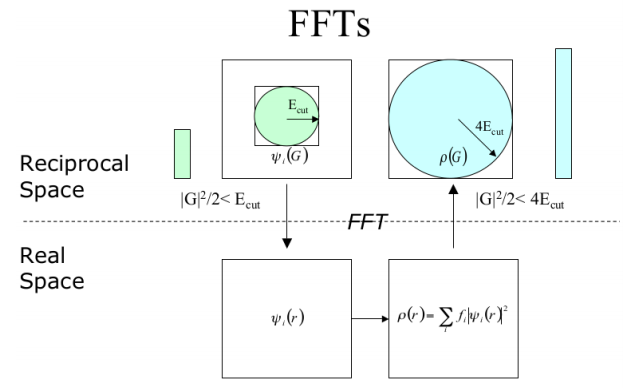
\includegraphics[scale = 0.6]{figs/D2/FFT.png}
      \caption{El cuadrado representa la caja (grilla) sobre la que se efectúa la FT. Para los orbitales KS sólo se requiere $\sfrac{1}{8}$ de la misma (izquierda), mientras que para la densidad de carga requiero  ocupar todavía más.}
      \label{fig:FFT}
  \end{figure}

\subsection{FFT}

  Mientras que el costo computacional de la FT convencional para $n$ partículas es tal que $t_{CPU} = \mathcal{O} (n^2)$, el costo para la transformada rápida de Fourier (FFT) va como $t_{CPU} = \mathcal{O} (n \log{n})$. Esto da lugar a una enorme mejora el los cálculos PW.

\subsection{Dual space technique}

  Teniendo
    $$H\psi = (T + V_{NonLoc} + V_{loc} + V_H + V_{xc})\psi$$

  se cumple que
    \begin{itemize}
      \item $T\psi$ es más fáci de clacularen el $G$-espacio: $t_{CPU} = \mathcal{O} (n)$
      \item $(V_{loc} + V_H + V_{xc})\psi$ es más fácil de calcular en el $R$-espacio: $t_{CPU} = \mathcal{O} (n)$
      \item $V_{NonLoc}\psi$ es fácil en ambos espacios siempre que el operador sea separable en proyectores: $t_{CPU} = \mathcal{O} (mn)$ siendo $m$ la cantidad de proyectores utilizados.
    \end{itemize}

  Con esto en mente, se utiliza la FFT para ir y volver entre el $R$-espacio y el $G$-espacio a conveniencia.

\subsection{Simetrización de la densidad de carga}

  La densidad de carga calculada por el código está no simetrizada:
    $$\tilde{n} (\vec{r}) = \sum_{k\in IBZ} \sum_v \omega_k \norm{\psi_{k,v} (\vec{r})}$$

  donde la suma corre sólo sobre estados ocupados y $k$-puntos simétricamente inequivalentes, los cuales pertenecen a la zona de Brillouin irreducible (IBZ), la cual es la 1BZ reducida por todas las operaciones de simetría del grupo puntual al que pertenece el cristal. Los coeficientes $\omega_k$ pesan la simetría: es la cantidad de $k$-puntos que son equivalentes a $k$ por simetría.

  \Obs{Tanto la grilla de $k$-puntos sobre la IBZ como los $\omega_k$ pueden ser calculados o provistos por el usuario.}

  La verdadera densidad de carga se obtiene via simetrización:
    $$n(\vec{r}) = \frac{1}{N_S} \sum_{n=1}^{N_S} \hat{O}_n \tilde{n} (\vec{r}) = \frac{1}{N_S} \sum_{n=1}^{N_S}  \tilde{n} (O_n^{-1} \vec{r})$$

  donde $\hat{O}_n$ es la $n$-ésima simetría del cristal y $O_n$ es la matriz de rotación asociada. Para grupos que contienen operaciones de simetría con traslaciones fraccionarias, lo anterior se generaliza a
    $$n(\vec{r}) = \frac{1}{N_S} \sum_{n=1}^{N_S}  \tilde{n} (O_n^{-1} \vec{r} - \vec{f}_n)$$

  siendo $\vec{f}_n$ la traslación fraccionaria con respecto al vector de red para la $n$-ésima operación.

  \Obs{En pw la simetrización es llevada a cabo en el $G$-espacio por lo que
    $$n(\vec{G}) = \frac{1}{N_S} \sum_{n=1}^{N_S}  \tilde{n} (O_n^{-1} \vec{G}) \exp{-i O_n^{-1} \vec{G}\cdot\vec{f}_n)}$$}

\subsection{Augmentation charge}

  Para USPP y PAW PP se agrega el término de augmentation charge. Así
    $$n^{aug} (\vec{r}) = \sum_{\mu,l,m} \braket{\psi_i}{\beta_l} Q_{\mu,l,m} (\vec{r}) \braket{\beta_m}{\psi_i}$$

  donde $\mu$ corre sobre los núcleos mientras que $\beta_l$ y $Q_{\mu,l,m}$ son funciones de corto alcance centradas en el átomo $\mu$.

  El primer término de $n (\vec{r})$, dado por $\norm{\psi_i (\vec{r})}^2$, se calcula fácilmente con la misma grilla de FFT utilizada en el cálculo de $H\psi$, conteniendo las componentes de Fourier del $G$-espacio hasta la energía cinética de $4E_{cut}$. El término de augmentation charge se calcula en una grillas más grande y densa, conteniendo $G$ hasta un cutoff mayor que $4E_{cut}$.

\subsection{Metales}

\subsubsection{Densidad de carga en metales}

  La manera más directa de calcular con metales es introducir un ensanchamiento de los niveles discretos. Así
    $$n(\vec{r}) = \sum_i f_i \norm{\psi_i (\vec{r})}^2 $$

  donde $f_i\in [0,1]$ son ocupaciones fraccionaraias dadas por
    $$f_i = \int_{\epsilon < \epsilon_F} \delta (\epsilon - \epsilon_i) d \epsilon \quad ; \quad \sum_i f_i = N_{\epsilon_F}$$

  y la energía de Fermi $\epsilon_F$ queda determianda por la condición $N_{\epsilon_F}  = N_{elec}$. El integrando $\delta(x)$ es la función (normalizada) de ensanchamiento. Aunque uno podría utilizar la función de Fermi-Dirac en principio, no es conveniente ya que se necesitaría una temperatura muy alta y la distribución tendría colas muy largas.
    $$\delta_{FD} (x) = \frac{1}{e^{x\beta} + 1}$$

\subsubsection{Energía en metales}

  La manera de calcular la energía es
    $$E_{KS} = \sum_i \int_{\epsilon < \epsilon_F} \epsilon \delta (\epsilon - \epsilon_i) d \epsilon = \tilde{E}_{KS} + \delta E_{met}$$

  donde
    $$\tilde{E}_{KS} = \sum_i \epsilon_i \int_{\epsilon < \epsilon_F}  \delta (\epsilon - \epsilon_i) d \epsilon = \sum_i f_i \epsilon_i
    \quad ; \quad
    \delta E_{met} = \sum_i \int_{\epsilon < \epsilon_F} (\epsilon - \epsilon_i) \delta (\epsilon - \epsilon_i) d \epsilon$$

  Esta contribución $\delta E_{met}$ aparece en el output como $smearin\ contrib.\ (-TS)\ \ [Ry]$.

\subsubsection{Funciones de ensanchamiento}

  Una posibilidad es la función Gaussiana normalizada
    $$\delta(x) = \frac{1}{\sigma \sqrt(\pi)} e^{-\frac{x^2}{\sigma^2}} \quad ; \quad \int \delta(x) = 1$$

  donde $\sigma$ (medido en Ry y escrito como $degauss$ en el input) da lugar a una temperatura ficticia $T=\sfrac{\sigma}{k_B}$ a la cual se corresponde un funcional de energía libre $E_{KS} [\sigma]$.

  Se puede ver que $E_{KS} [\sigma] \propto \sigma^2$ por lo que a mayor $\sigma$ (lo cual hace falta para una convergencia rápida de $k$-puntos) dan lugar a mayores diferencias entre la energía \emph{libre} y la real.

  \Obs{A mayor $\sigma$, menor es la cantidad de $k$-puntos necesarios. Lo ideal sería minimizar ambas situaciones en sentido de que la convergencia sea más económica.}

  Otra posibilidad es utilizar los \emph{smearing fríos} de Methfessel-Paxton (MP) o de Marzari-Vanderbilt (MV). En este caso el término cuadrático desaparece haciendo que $E_{KS} [\sigma] \propto \sigma^4$, dando lugar a una mejor convergencia (ver http://theossrv1.epfl.ch/Main/ElectronicTemperature). A pesar de esto:
    \begin{itemize}
      \item Con MP se pueden dar ocupancias negativas o mayores a 1.
      \item Con MV las ocupacias son no negativas, pero igual pueden superar la unidad.
      \item En ambos casos no se asegura que $N(\epsilon)$ sea una función monotónica. En consecuencia, la energía de Fermi puede no estar unívocamente definida.
    \end{itemize}

\subsection{Magnetización}

  En el caso no polarizado, cada orbital se encuentra doblemente ocupado y la densidad de carga será entonces
    $$n (\vec{r}) = 2 \sum_i f_i \norm{\psi_i (\vec{r})}^2$$

  En el caso de magnetización colinear (LSDA), cada orbital tiene o spin up o spin down. Esto da lugar tanto a una densidad de carga como a una magnetización
    $$n (\vec{r}) = n_{+} (\vec{r}) + n_{-} (\vec{r}) \quad ; \quad m (\vec{r}) = n_{+} (\vec{r}) - n_{-} (\vec{r})$$
    $$n_{\pm} (\vec{r}) = \sum_i f_{i, \pm} \norm{\psi_{i, \pm} (\vec{r})}^2$$

  \Obs{En QE el índice $\pm$ está oculto en el indexado de los $k$-puntos: se dobla la cantidad de $k$-puntos, donde el primer conjunto corresponde a spin up y el segundo conjunto a spin down.}

  Para el caso más general donde la magnetización es no colineal, la base de PWs debe ampliarse con los spinores quedando
    $$\Psi (\vec{r}) = \psi_+ \chi_+ + \psi_- \chi_-$$

  Tenemos entonces la densidad de carga
    $$n (\vec{r}) = \sum_i f_i \left[ \norm{\psi_{i,+} (\vec{r})}^2 + \norm{\psi_{i,-} (\vec{r})}^2 \right]$$

  y un vector de magnetización
    $$\vec{m} (\vec{r}) = \sum_i f_i \Psi_i^{\dagger} (\vec{r}) \vec{\sigma} \Psi_i (\vec{r})$$

  donde $\vec{\sigma}$ corresponde a las matrices de Pauli.

\subsection{Potenciales y energía}

  Los siguientes potenciales de largo alcance son divergentes (separadamente) para $\vec{G} = 0$: $V_{Har}$ y $V_{loc}$. Esto se da sólo cuando hay cargas, ya que cuando el sistema es neutro no hay divergencia en dicho origen. Los demás térmios son de corto alcance ($V_{xc}$ y $V_{NonLoc}$).

  A partir de los potenciales la energía total se escribe como
    $$E = E_{KS} - E_{Har} - \int n(\vec{r}) V_{xc} d\vec{r} + E_{xc} + E_{Ewald}$$

  donde
    \begin{itemize}
      \item $E_{KS} \rightarrow$ suma de las contribuciones monoelectrónicas de los orbitales KS, incluyendo la energía electrón-ión.
      \item $E_{Har} \rightarrow$ energía electrónica electrostática con la singularidad levantada. Se resta porque se considera dos veces en $E_{KS}$.
      \item $E_{KS} \rightarrow$ se extrae de $E_{KS}$ y se lo agrega como $E_{xc}$.
      \item $E_{KS} \rightarrow$ interacción interiónica en presencia de un fondo neutralizante.
    \end{itemize}

\subsection{Electrostática en PBC}

  Como consecuencias de la periodicidad se tiene que
    \begin{itemize}
      \item La carga neta por unidad de celda debe ser nula o la energía será divergente.
      \item Todos los potenciales son periódicos con la red, no pudiendo utilizar campos eléctricos macroscópicos.
      \item El cero de la energía es arbitrario.
      \item El momento dipolar por celda unitaria suele estar mal definidos.
    \end{itemize}

  En el caso de sistemas cargados, la singularidad en el origen del $G$-espacio se redefine la energía con una redefinición del potencial en dicho punto, por lo que la energía es dependiente de la elección. Además la comparación entre energías con diferente $N_{elec}$ para el mismo sistema no es confiable. Por último no hay garantías de que la optimización estructural arroje resultados confiables.

  Si el sistema es finito (sea cargado o no), \emph{i.e.} no es periódico, se pueden aplicar diferentes trucos que corrigen la energía o el potencial y la energia.

\subsection{Superficies polares: correción dipolar}

  Las superficies polares tienen un dipolo. Al usar un slab en PBC, el dipolo produce interacciones ficticias que caen muy lentamente entre el sistema real y sus imágenes. Para remover esta interacción espúrea uno puede agregar un dipolo que compense la situación en la región vacía del esapcio.

  \Obs{Ver trabajo: potential profile for MoS2 on Au surfaces (Pedram Khakbaz et al, Solid State Electronics, in press).}

\section{Q\&A}

  \definicion{Sobre el uso del smearing en la silica}

  The most likely source of trouble in your case is the fact that models of polar/non-polar interfaces easily get charged and thus develop unphysical electric fields across the sample. An analysis of the intermediate charge-density distribution and/or of the resulting electrostatic potential may help  diagnose the problem. The cure is likely a recostruction of the interface to make it neutral

  I think one problem is that you used Gaussian broadening as a smearing function. It is known that this broadening function leads to a strong dependence of the total energy on sigma. For this reason, the "cold" smearing of Marzari-Vanderbilt has been invented: the energy depends less on sigma, for small sigma

  You might want to look at chapter 4 of Marzari's PhD thesis, from here http://theossrv1.epfl.ch/Main/Theses?action=download\&upname=Marzari\_thesis\_1996.pdf

  \definicion{How could I choose the best smearing depending on the material? For example for iron is usual to use M-V instead M-P? Also, is there a way to predict the value of degauss?}

  You need to do a test. The advantage of M-V with respect to M-P smearing is that the occupation numbers are guaranteed to be always non-negative with M-V. As a rule of thumb, M-V is always a good choice, except if your aim is to simulate real temperature effects on the electrons. In that case, you must use Fermi-Dirac smearing.


  \definicion{How do we choose the kpoints for the cutoff convergence tests?}

  a mesh dense enough for the calculation to  converge but the smaller as possible. As long as you use the same mesh the convergence test is valid, no  matter what mesh you use.

  Typically any reasonable k-point mesh will do the job. Convergence tests can be done one parameter at the time, fixing reasonable values of the other parameters. For metals, however, the value of the broadening and the k-point grid are correlated.

  \definicion{what is the unit of "Ry" in ecut}

  12*13.6058 eV

  \definicion{What's the criterion to choose the best ecutwfc?}

  It depends on the accuracy that you desire for the computed quantity. Also for the k-points mesh.

  \definicion{In the case of Al (metal), the converged kpoints are clear, but how to determine an accurate degauss value? so then should i choose the smallest value of the "plateau" in the middle of the figure?}

  in principle it should be as small as possible but not so small as to cause convergence problems. Something like that you can choose.  better to be more conservative

  Wait a minute! In a metal, the function which you need to integrate over the Brillouin zone is like a "step function" at the Fermi surface. The higher you choose the degauss, the smoother that function becomes. Therefore, for a higher value of degauss you need less k-points (because the function to be integrated is smoother) and inversely, a very small value of degauss entails a huge number of k-points.

  In principle you can create a graph like this, where for every value of degauss you plot the energy (with a converged set of k-points, which might be different for different degaus values, see above). Then, you decide which value of the energy is "good enough" for your needs.

  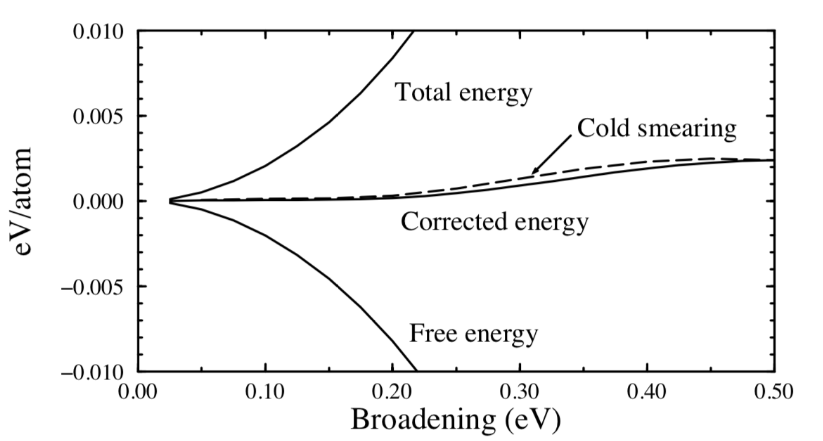
\includegraphics[scale = 0.6]{figs/D2/smearing.png}

  \definicion{I have seen the discussion about relax in zoom. When we should use "relax" instead of "vc-relax"? I have seen  "relax " in papers related to molecules ( with complex carbon structures) is this a correct approach?}

  in general I'd use vc-relax only to obtain the DFT lattice parameters of the crystal bulk structure, which are typically slightly different than the experimental ones. For trying different atomic configurations in the cell relax should be used (after you already obtained appropriate cell parameters) , but it will be discussed tomorrow yes

  \definicion{if we have a ferromagnetic system, how do we know in which direction the magnetization vector is pointing? Where do we find the components of the magnetization vector?}

  In order to know this information, you need to setup a non-collinear calculations with spin-orbit-  in  this way you can explore different directions of the magnetitazion and
  the relative energy differences for each specific direction you fix in
  the input file.
  You can even setup a constrained magnetic moment calculations to adress these energy differences-
  When
  performing non-collinear calculations, in the output file you access to
  the cartesian components of the magnetization for each magnetic atoms-

  \definicion{In the case of a defect calculation, should I first converge the supercell size or is it better to converge first ecut, kpoints, etc., on a smaller cell and do the cell size convergence after?}

  a smaller cell is better, but you have to keep the density of k-points consistent.

  I think its better if you first converge the  ecut and kpoints and than the supercell size.

  \definicion{Thank you! Regarding the reducing number of the k points, if the k-points converged for 8x8x8 in a 2x2x2 supercell and I need a 3x3x3 supercell, which k-points can I use (as it is not a divisor)? Should I round up (6x6x6)?}

  closest integer, preferably rounded up

  \definicion{Question: What is the criteria for cartegorizing a magnetic material as antiferromagnetic or ferromagnetic with respect to the total magnetization, absolute magnetization and magnetic moment?}

  For ferromagnetic materials, the total and absolute magnetization are (almost) the same. For AFM, total magnetization is 0, absolute magnetization is not.

  \definicion{I have a question. If we use very high E\_cut in PAW e.g. 120Ry with E\_rho = 4E\_cut, will the result be acceptable?}

  Likely yes, but it is not a smart (that is: efficient) choice. The higher Ecut means the more cost of CPU.


  \definicion{Another question is, If I do not have metal, is better to use gauss smearing?}

  For insulators you usually don’t need smearing. In case if you use it for getting faster convergence use gaussian smearing with a very small degauss value.

  \definicion{Why did the professor  use starting magnetization 0.6 and -0.6 for AFM iron? My question is about the number, can I use 0.5 and -0.5 or even 1 and -1? Is there  a restricción?}

  you can also start with 0.5. it will converge at the end. If you have rough idea about the number, the simulation will be faster. What you provide is just an initial guess. The code will eventually converge to you different value

  \definicion{I got some doubts about testing convergence. Suppose I've got a slab of an insulator inside a supercell with, let's say, 20 atoms (10 of element A and 10 of element B) and it's the minimal slab I need (I can create greater surfaces multiplaying this "unit" in the xy plane)
  1. How should I run the tests for the cutoffs? I mean should I sweep values for the whole slab or how?
  Suppose now that in order to converge I need to add smearing.
  2. What should be my "first choice" since it's an insulator: gauss or MV?
  3. Since it's not a metal I understand that the smearing contribution should be the least possible. Can I apply the same criterion we used in the hands-on (there was a 3D system and here it is a slab)? There we said that the we considered the convergence achieved with 1mRy/atom so here I should seek for a value of smearing contribution to be lesser than 20mRy?}

  1.) the ecutwfc and ecutrho are properties of the pseudopotential, so you only have to test it for each atomic type in your system (2 in your example), you can do the test for the isolated atom or the bulk structure of the crystal, then you use the highest/hardest cutoff for your supercell calculation. the cell size shouldn't matter for the ecut, what matters is that the energy doesn't change once you increase the cutoff further

  2.) the smearing is a bit more difficult, but you can use mv/mp for insulators as well, but the smearing there should be really small (no bigger than 0.01 Ry), basically you add it only to help in the convergence, once you choose it keep it the same for all calculations (supercells included), so in principle you can determine it for the bulk of the insulator, note that the 0.001 Ry/atom is the criterion for the cutoff not the smearing typically.

  in any case keep an eye on the smearing contribution written in the output and make sure its not significant and at least consistent between different calculations

\section{Hands-on}

    \definicion{Topic:} SCF calculations + post-processing – part 2. Exercises.

    \definicion{Speaker:}	Anton KOKALJ (Jožef Stefan Institute, Slovenia).

\subsection{Si}

\subsubsection{Objetivo}

  Estudiar la convergencia de cálculos pw.x para diferentes Si bulk: primero se estudia la convergencia del cutoff para las funciones de onda ($ecutwfc$) y luego la convergencia para los puntos $k$.

  Las pruebas de convergencia se llevan a cabo haciendo una siere de cálculos variando algún parámetro. Para esto se pueden utilizar shell scripts o PWTK scripts. La diferencia entre estos peuede observarse al comparar, por ejemplo, ex1.ecutwfc.classic/ecutwfc.sh con ex1.ecutwfc/ecutwfc.pwtk, respectivamente.

  La lógica a seguir es la siguiente:
    \begin{enumerate}
      \item Convergencia de la base ($ecutwfc$).
      \item Convergencia de los puntos $k$, utilizando el valor óptimo de $ecutwfc$.
      \item Convergencia del parámetro de red, utilizando los valores óptimos para $ecutwfc$ y la grilla de puntos $k$.
      \item Calcular la estructura de bandas, utilizando los valores óptimos para $ecutwfc$, la $k$-grilla y el parámetro de red.
    \end{enumerate}

\subsubsection{Pasos}

    \begin{enumerate}
      \item Convergencia de $ecutwfc$: correr alguno de los siguientes comandos a gusto.
        \begin{verbatim}
          ./ecutwfc.sh         (shell)
          pwtk ecutwfc.pwtk    (PWTK)
        \end{verbatim}
      \item Convergencia de $k$-grid.
        \begin{verbatim}
          pwtk kpoints.pwtk
        \end{verbatim}
      \item Convergencia del parámetro de red: agregar parámetros necesarios al script antes de correr. Primero corre pw.x y luego ev.x para obtener el parámetro de red y el módulo de Young recurriedno a la ecuación de estado de Murnaghan.
        \begin{verbatim}
          pwtk alat.pwtk
        \end{verbatim}
      \item Estructura de bandas: agregar parámetros necesarios al script antes de correr. Luego de la corrida, poner la energía de Fermi adecuada en el archivo plot.gp. Regraficar la estructura de bandas.
        \begin{verbatim}
          pwtk bands.pwtk
          grep 'highest occupied level' pw.Si.scf.out
          gnuplot plot.gp
        \end{verbatim}
    \end{enumerate}

\subsubsection{Resultados: Si}

  Para los cálculos se utilizaron NCPP con LDA (PZ) como funcional: Si.pz-vbc.UPF.

  Para examinar cómo avanza la autoconsistencia, podemos ejecutar
  \begin{verbatim}
    grep -e "total energy" -e estimated output\_file.out
  \end{verbatim}

  Notar que hay 9 elecctrones dentro de la celda ya que hay 2 átomos por celda con 4 electrones cada uno. Como el sistema es no magnético y es aislante, sólo se computan las 4 ($=\sfrac{8}{2}$) bandas de valencia (estados KS) más bajas.

  Es recomendable usar PWTK ya que está hecho explícitamente para funcionar con QE: la sintáxis se mantiene como en el input original.

  \begin{figure}[H]
      \centering
      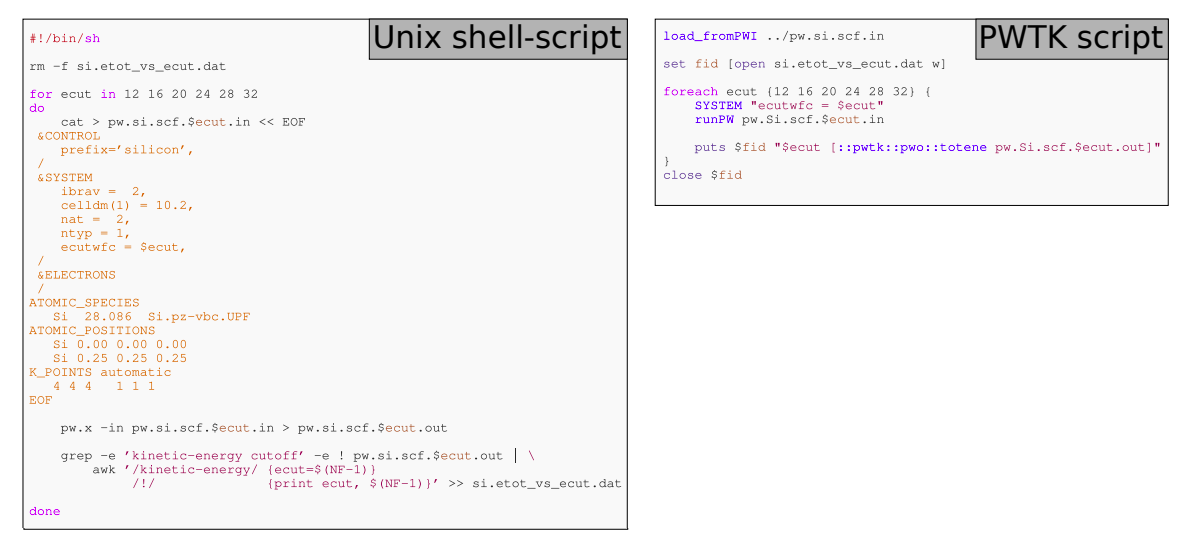
\includegraphics[scale = 0.4]{figs/D2/shellvspwtk.png}
      \caption{Comparación de un script en shell y uno en PWTK.}
  \end{figure}

  Los PWTK scripts son Tcl-scripts donde:
    \begin{itemize}
      \item Se mantienen los nombres de las namelists y las cards, salvo contadas excepciones. Su contenido debe ir entre corchetes (pensarlo como una función de C).
      \item Se pueden escribir tanto números como expresiones matemáticas, pero no debe haber espacios que separen los términos y factores de la expresión.
      \item Se puede indexar usando, por ejemplo, los nombres de los átomos.
      \item Es casesensitive, pero el orden de las namelists y las cards no es importante.
      \item Las variables de los namelists pueden configurarse on-the-fly.
      \item Tanto las namelists como las cards pueden ser llamadas múltiples veces. Sin embargo, PWTK no las considera de igual forma: las cards son tratadas en overwrite mode, mientras que las namelists son tratadas en append mode.
      \item Para desactivar una variable dentro de una namelist basta con darle un valor vacío, \emph{i.e.} no poner nada después del igual.
    \end{itemize}

    Algunas de las funciones que se usan de PWTK en este hands-on son:
      \begin{itemize}
        \item \textbf{load\_fromPWI:} carga input data desde un input de pw.x existente.
        \item \textbf{pwo\_totene:} devuelve la energía total de un output de pw.x.
        \item \textbf{seq:} devuelve una secuencia de números. El primero y el último número son los extremos del intervalo (cerrado). El valor del medio indica el salto.
        \item \textbf{runPW / runPP / runDOS / runPROJWFC:} construye un input file del programa dado (PW, PP, DOS o PROJWFC) y corre el cálculo.
      \end{itemize}

    Respecto al barrido de $ecutwfc$, asumimos que el sistema es convergente cuando la diferencia entre los valores de energía total entre dos mediciones sucesivas de $ecutwfc$ es menor que $1\ \sfrac{mRy}{\sfrac{atom}{cell}}$. En este caso tenemos 2 átomos por celda así que serían $2\ mRy$. De la gráfica podemos pensar que 24 Ry sería suficiente. En números:
      $E_{tot} (24 Ry) = -15.8508\ Ry \wedge E_{tot} (20 Ry) = -15.8475\ Ry \Rightarrow \Delta E_{tot} = 0.0033\ Ry = 3.3\ mRy$

      $E_{tot} (24 Ry) = -15.8508\ Ry \wedge E_{tot} (28 Ry) = -15.8519\ Ry \Rightarrow \Delta E_{tot} = 0.0011\ Ry = 1.1\ mRy$

    Se concluye entones que el valor óptimo es $ecutwfc = 24$.

      \begin{figure}[H]
          \centering
          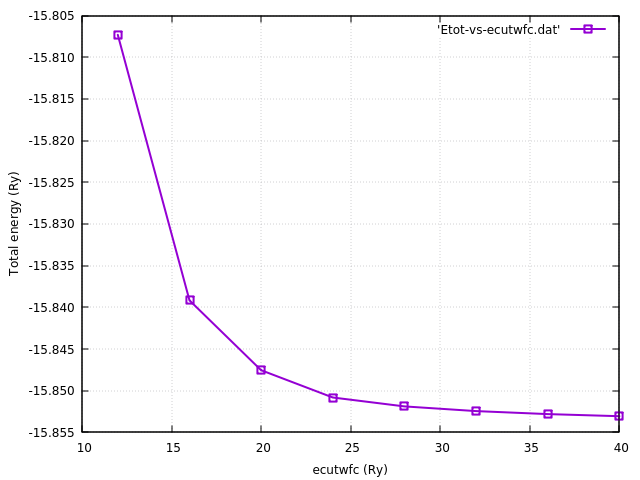
\includegraphics[scale = 0.6]{figs/D2/Si_ecutwfc.png}
          \caption{Barrido de $ecutwfc$ para Si bulk.}
      \end{figure}

    Ahora hacemos el barrido de la $k$-mesh. Consideramos el mismo criterio de convergencia.
      $E_{tot} (222) = -15.7945\ Ry \wedge E_{tot} (444) = -15.8073\ Ry \Rightarrow \Delta E_{tot} = 0.0128\ Ry = 12.8\ mRy$

      $E_{tot} (444) = -15.8073\ Ry \wedge E_{tot} (666) = -15.8076\ Ry \Rightarrow \Delta E_{tot} = 0.0003\ Ry = 0.3\ mRy$

    Se concluye entones que el valor óptimo es $4\ 4\ 4$.

      \begin{figure}[H]
          \centering
          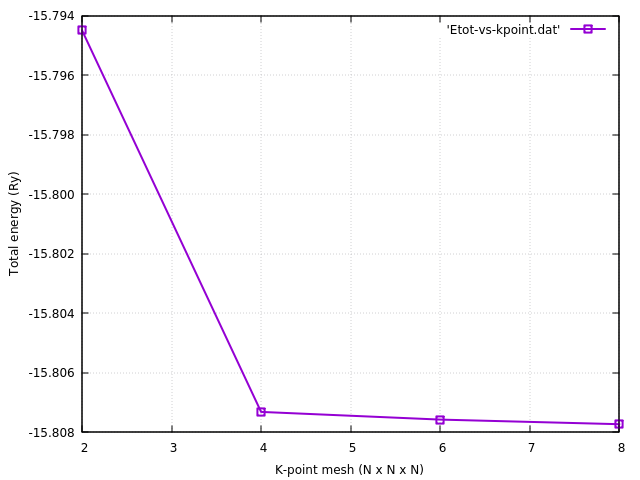
\includegraphics[scale = 0.6]{figs/D2/Si_k.png}
          \caption{Barrido de $k$-mesh para Si bulk.}
      \end{figure}

    \Obs{La convergencia de los puntos k no es necesariamente monotónica ya que no existe ningun principio variacional con respecto al número de puntos k.}

    Ahora analizamos el parámetro de red. El equilibrio en el caso del Si queda determinado por aquel parámetro de red que minimiza la energía ya que no hay fuerzas actuando sobre los átomos dada la simetría.

    \Obs{La ausencia de fuerzas debida a la simetría puede chequearse haciedno $tprnfor=.tru.$ en \&CONTROl.}

    De la gráfica vemos que es $10.2\ Bohr$. Siendo más precisos, la ecuación de estado nos dice que es $10.2090\ Bohr$ y el módulo de Young es $934\ kbar$.

    A partir de los resultados de la ecuación de estado, notamos además que para parámetros de red menores al óptimo, la energía total es menor que la entalpía. Lo opuesto ocurre para parámetros de red mayores al óptimo.

      \begin{figure}[H]
          \centering
          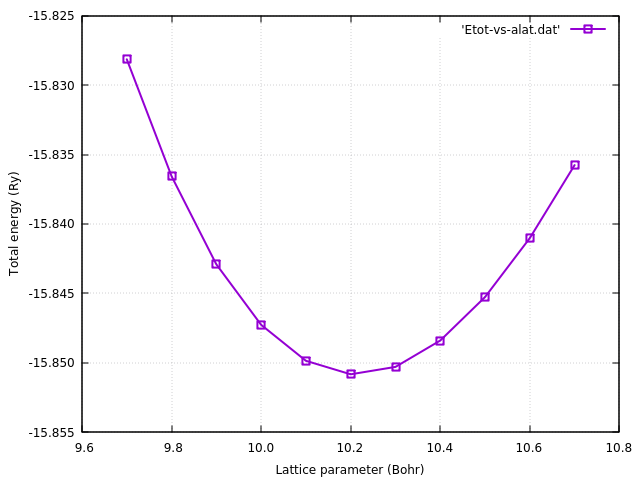
\includegraphics[scale = 0.6]{figs/D2/Si_alat.png}
          \caption{Barrido del parámetro de red para Si bulk.}
      \end{figure}

      \begin{figure}[H]
          \centering
          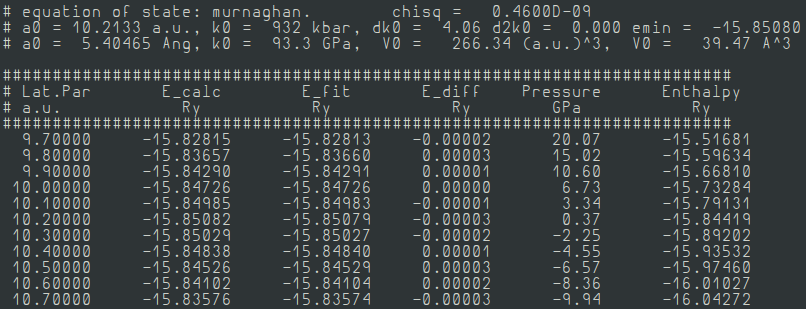
\includegraphics[scale = 0.6]{figs/D2/Si_mur.png}
          \caption{Resultados del fiteo utilizando la ecuación de estado.}
      \end{figure}

    Para hacer el cálculo de bandas, no podemos usar el mesh corrido, sino los valores serán erróneos: no estaríamos incluyendo el punto $\Gamma$.

    \begin{figure}[H]
        \centering
        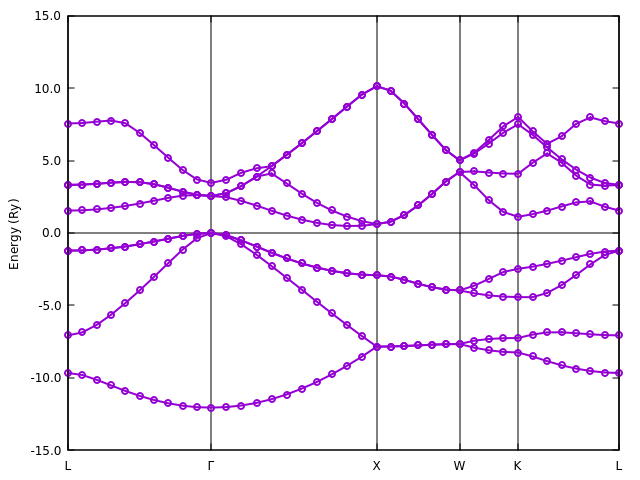
\includegraphics[scale = 0.6]{figs/D2/Si_bands.png}
        \caption{Estructura de bandas para Si bulk.}
    \end{figure}

  Al analizar las curvas de energía total en función del parámetro de red para diferentes $k$-mesh y $ecutwfc$ vemos que:
    \begin{itemize}
      \item Para un mismo $ecutwfc$, la energía no es tan sensible al $k$-mesh: con 2x2x2 es muy mala la convergencia, pero ya con 4x4x4 se estabiliza.
      \item A medida que aumentamos $ecutwfc$, las curvas se van desplazando hacia valores más negativos de energía.
    \end{itemize}

  Al comparar los $k$-mesh volvemos a elegir 4x4x4. Al comparar los mínimos, vemos que la elección de 24 Ry fue acertada.

  \begin{figure}[H]
      \centering
      \subfigure[]{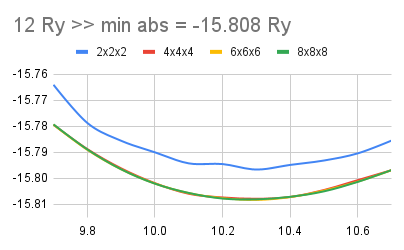
\includegraphics[scale = 0.55]{figs/D2/alat/12.png}}
      \subfigure[]{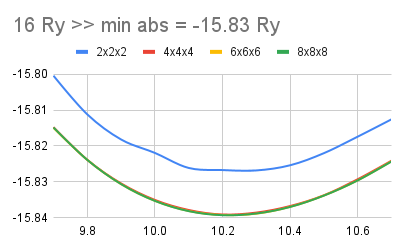
\includegraphics[scale = 0.55]{figs/D2/alat/16.png}} \\
      \subfigure[]{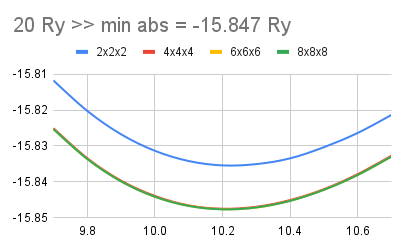
\includegraphics[scale = 0.55]{figs/D2/alat/20.png}}
      \subfigure[]{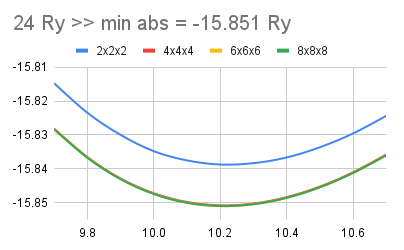
\includegraphics[scale = 0.55]{figs/D2/alat/24.png}} \\
      \subfigure[]{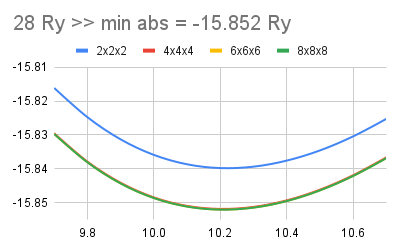
\includegraphics[scale = 0.55]{figs/D2/alat/28.png}}
      \subfigure[]{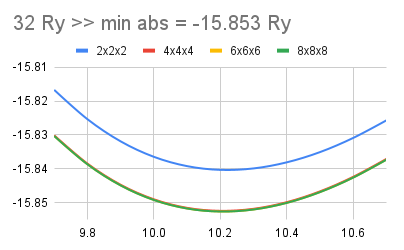
\includegraphics[scale = 0.55]{figs/D2/alat/32.png}} \\
      \subfigure[]{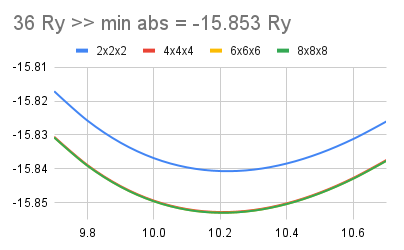
\includegraphics[scale = 0.55]{figs/D2/alat/36.png}}
      \subfigure[]{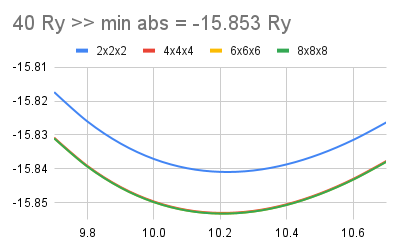
\includegraphics[scale = 0.55]{figs/D2/alat/40.png}} \\
      \caption{Energía en total en función del parámetro de red para diferentes cutoff y diferentes $k$-mesh.}
  \end{figure}


\subsection{Al}

\subsubsection{Objetivo}

  Cálculo de sistemas metálicos: Al bulk.

  Se explora diferentes esquemas de smearing: cómo hacerlo y hasta dónde. Se plotea la densidad de carga electrónica.

\subsubsection{Pasos}

    \begin{enumerate}
      \item Explorar qué hace el smearing con función de ensanchamiento Gaussiana. Una vez que corra, edirar el .pwtk y agregar más puntos de degauss, como 0.15 ó 0.2, dentro del foreach. Para evitar volver a correr lo ya corrido, encender el modo $restart$ (descome $\#restart\ true$).
        \begin{verbatim}
          pwtk degauss.pwtk
        \end{verbatim}
      \item Calcular la densidad de carga (chdens).
        \begin{enumerate}
          \item \textbf{1-chdens.pwtk:}
            Calcular la densidad de carga de valencia. Editar con las variables adecuadas antes de correr. Ver la densidad de carga con xcrysden.
            \begin{verbatim}
              pwtk 1-chdens.pwtk
            \end{verbatim}
          \item \textbf{2-chdens-paw.pwtk:}
            Calcular la densidad de carga all-electron tanto de valencia como total, mediante el uso de PAWPP. Ver en xcrysden.
            \begin{verbatim}
              pwtk 2-chdens-paw.pwtk
              xcrysden --xsf all-electron-VALENCE-chdens.xsf -s state2.xcrysden
              xcrysden --xsf all-electron-total-chdens.xsf  -s state2.xcrysden
            \end{verbatim}
        \end{enumerate}
    \end{enumerate}

\subsubsection{Resultados: Al}

Aunque Al es más simple que Si ya que tiene sólo un átomo por celda dentro de una FCC, se trata de un metal: no será suficiente con sólo conocer las bandas de valecias y pocos puntos k.

El barrido de parámetros es tridimensional: se analizan los puntos k, el tipo de smearing y el valor propio del smearing que se utiliza.

Cuando usamos $g$ (gaussian) vemos que la mesh 4x4x4 no es útil para Al como lo era para Si. A mayor smearing, las curvas convergen unas a otras. Con esto en mente, podríamos usar smearing más altos y una mesh con menos resolución. Cuando usamos $m-p$ o $m-v$ queda claro que la energía no depende tan fuertemente del smearing como en el caso anterior, permitiendo una convergencia más rápida y segura. En el caso del aluminio tenemos entonces que una buena convergencia podría alcanzarse usando $m-p$ o $m-v$ con un mesh 12x12x12 y un $degauss$ entre 0.01 y 0.05 Ry.

El ensanchamiento no puede reducirse demasiado: los niveles energéticos deben tener cierta superposición (es un metal) o de lo contrario la ventaja de hacer smearing se terminaría perdiendo. En otras palabras: valores de degauss muy altos empiezan a romper todo.

  \begin{figure}[H]
      \centering
      \subfigure[]{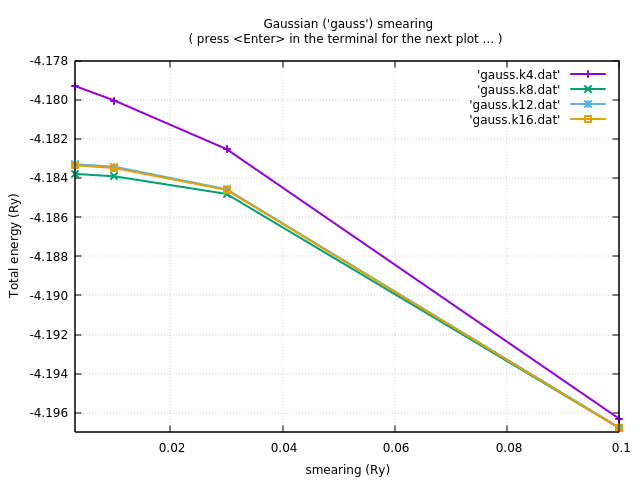
\includegraphics[scale = 0.45]{figs/D2/Al_gauss.png}}
      \subfigure[]{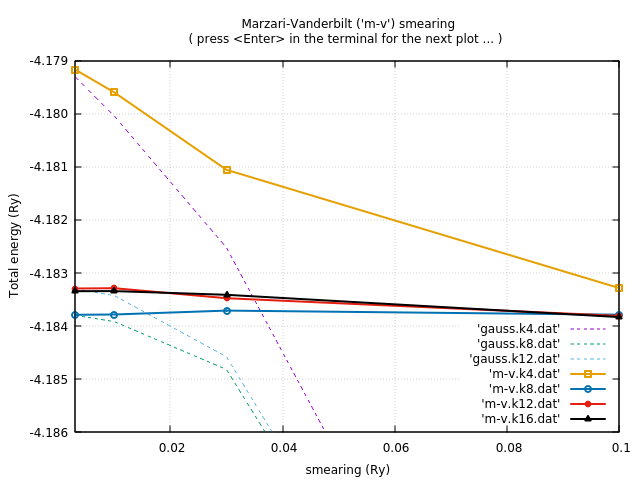
\includegraphics[scale = 0.45]{figs/D2/Al_mv.png}}
      \subfigure[]{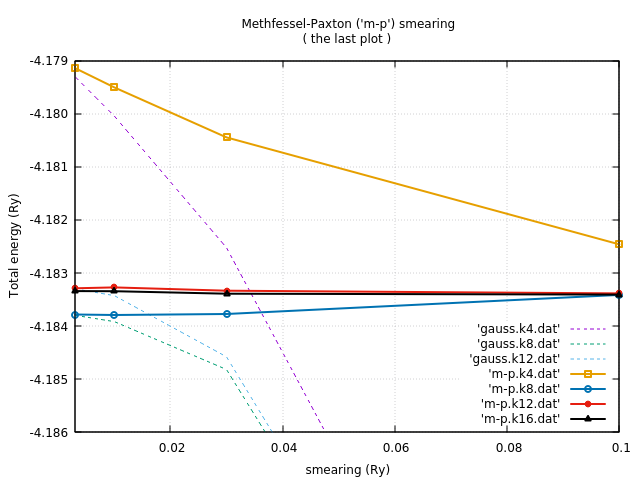
\includegraphics[scale = 0.45]{figs/D2/Al_mp.png}}
      \caption{Energía total en función del smearing y el ancho de smearing utilizado, variando la cantidad de puntos K. Las ocupaciones son: g (a), m-v (b) y m-p (c).}
  \end{figure}

  Dejando de lado los test de convergencia, vamos a ver cómo hacer un post-processing, determinando la densdiad de carga. La calculamos con dos potenciales diferentes:
    \begin{itemize}
      \item Un PP: Al.pz-vbc.UPF
      \item Un PAWPP para hacer un all-electron: Al.pbe-n-kjpaw\_psl.1.0.0.UPF
    \end{itemize}

  Las corridas con all-electron requieren cutoff gigantes (ecutrho ~ 1000 Ry). A partir de las figuras vemos que usando PP no hay electrones en torno a los núcleos, sino sólo en zonas intersticiales. Esto es por la manera en la que justamente construimos los PP. Para el caso del all-electron, se grafica valencia y full según el input del pp.x que le demos ($plot\_num$). En este caso sí se aprecia carga en torno al núcleo: es totalmente brillante debido a la alta concentración y localización de los electrones del core.

  \begin{figure}[H]
      \centering
      \subfigure[]{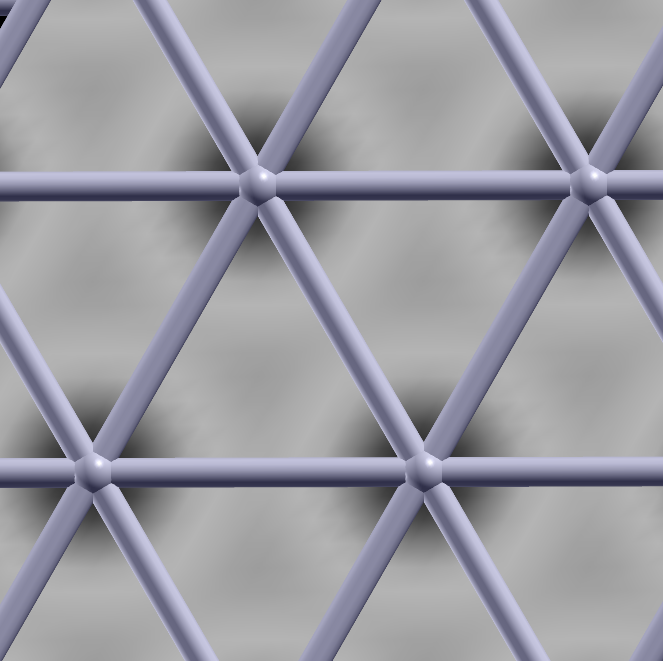
\includegraphics[scale = 0.35]{figs/D2/Al_chdens1.png}}
      \subfigure[]{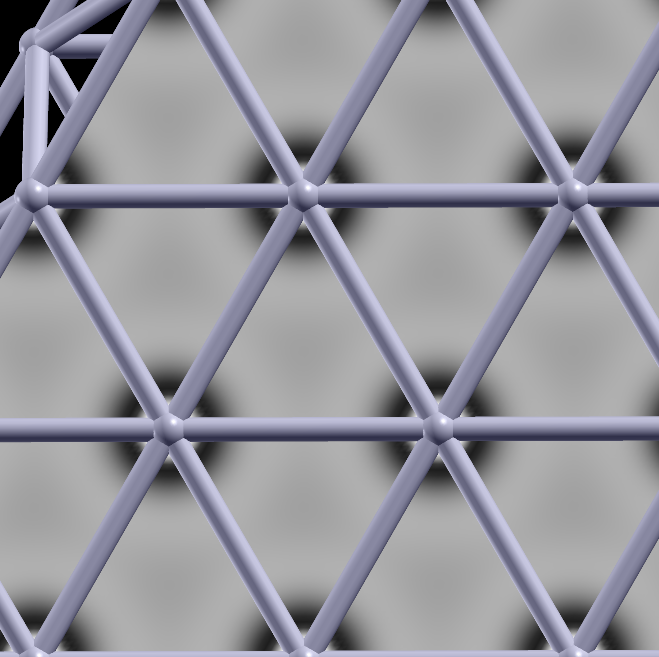
\includegraphics[scale = 0.35]{figs/D2/Al_chdens2_val.png}}
      \subfigure[]{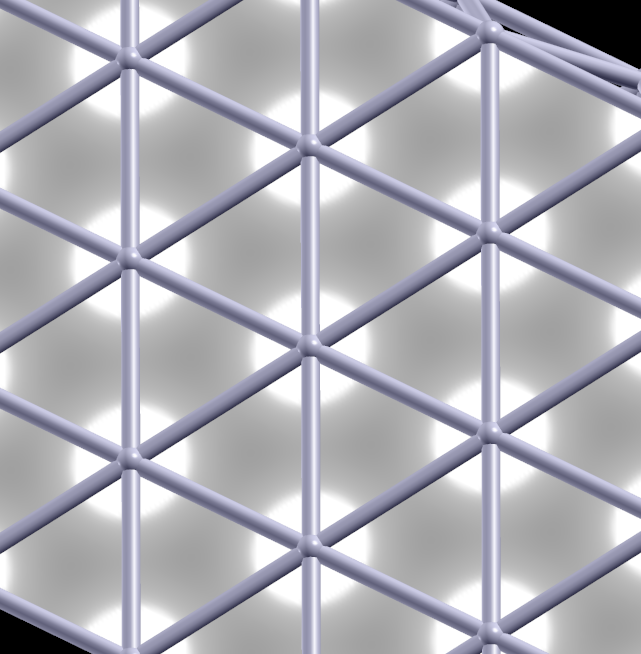
\includegraphics[scale = 0.35]{figs/D2/Al_chdens2_total.png}}
      \caption{Densidad de carga obtenida a partir de dos potenciales diferentes. Negro implica que no hay cargas y cuanto más brillante, mas carga hay. En (a) se usa el PP mientras que en los otros se usan el all-electron: (b) sólo valencia y (c) todo.}
  \end{figure}

\subsection{Fe}

\subsubsection{Objetivo}

  Realizar cálculos con sistemas magnéticos (bulk de Fe tanto ferromagnetico como antiferromagnetico). Aprender criterios de convergencias para USPP: el parámetro dual. Plotear DOS total y proyectada (PDOS) sobre los orbitales s y d.

\subsubsection{Pasos}

  Las diferencias entre los códigos ferromagnetico y antiferromagnetico pueden verse con
  \begin{verbatim}
    diff pw.fe\_fm.scf.in pw.fe\_afm.scf.in
  \end{verbatim}

  Los cálculos se pueden correr con
  \begin{verbatim}
    pw.x < pw.fe\_fm.scf.in > pw.fe\_fm.scf.out
    pw.x < pw.fe\_afm.scf.in > pw.fe\_afm.scf.out
  \end{verbatim}

  Analizar los outputs, prestando atención a los valores total/absolute magnetization en ambos casos.

    \begin{enumerate}
      \item Realizar un test de convergencia específico para USPP.
        \begin{verbatim}
          pwtk ecut.pwtk
        \end{verbatim}
      \item Calcular y plotear DOS y PDOS sobre OA s y d. Antes de correr, ingresar los valore adecuados de las variables necesarias. Luego poner el valor correcto de la energía de Fermi en plot.gp para después hacer el plot.
        \begin{verbatim}
          pwtk dos.pwtk
          grep 'Fermi energy' pw.Fe.nscf.out
          gnuplot plot.gp
        \end{verbatim}
    \end{enumerate}

\subsubsection{Resultados: Fe}

  En la siguiente figura se aprecia la diferencia entre ambos archivos, siendo primero el ferromagnetico y el segundo el antiferromagnetico.

    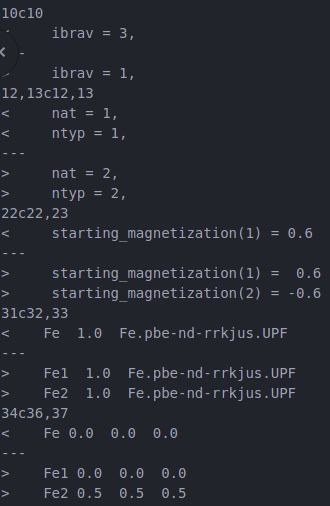
\includegraphics[scale = 0.45]{figs/D2/Fe_diff.png}

  Como vamos a usar un USPP (Fe.pbe-nd-rrkjus.UPF) debemos analizar la convergencia del $ecutrho$ también: tener $dual=4$ no será suficiente.
    $$dual = \frac{ecutrho}{ecutwfc}$$

  \Obs{Se puede estudiar también la variación del resultado respecto a la CI de la magnetización.}

  Al correr ambos  programas vemos que para el caso ferromagnetico la magnetización total es de 2.29 Bohr mag/cell y la absoluta es de 2.45 Bohr mag/cell, mientras que para el caso antiferromagnetico la total es 0 y la absoluta es 4.13 Bohr mag/cell.

  Ahora vamos a analizar la convergencia de los cutoffs con el caso ferromagnetico. Para ello se hace un barrido de dual y, para cada uno de ellos, se prueban diferentes ecutwfc. Vemos que para un dual de 4 tenemos una curva, pero para los duales 8 y 12 las curvas coinciden. Si queremos usar el dual de 4 debemos usar $ecutwfc > 40$; en cambio con los otros duales podemos usar $ecutwfc = 25$. En el código se hacen muchísimas más operaciones con las funciones de onda que con las densidades de carga, por lo que si usamos un $ecutwfc$ más chico el cálculo irá nás rápido.
    \begin{figure}[H]
        \centering
        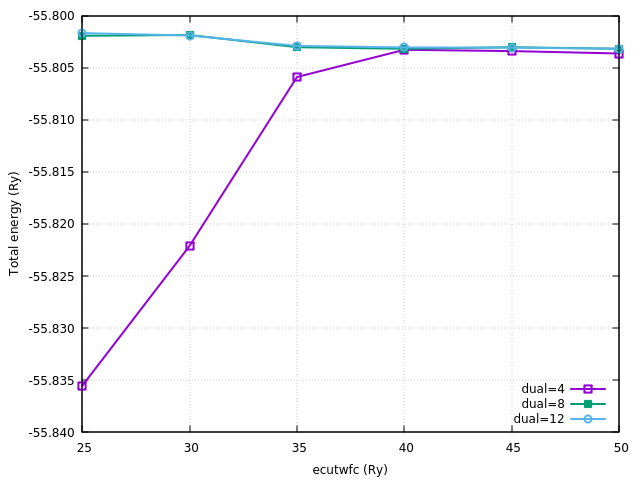
\includegraphics[scale = 0.45]{figs/D2/Fe_fm_dual.png}
        \caption{Variación de la energía total en función del dual para Fe ferromagnetico.}
    \end{figure}

  Ahora vamos a graficar DOS y PDOS, también para el caso ferromagnetico. Recordamos que necesitamos una $k$-mesh más densa. Además $occupations = 'tetrahedra'$ suele ser útil para este tipo de cálculos. En la DOS vemos que hay más estados ocupados con spin up que down. En la PDOS vemos que
    \begin{itemize}
      \item Las bandas s son muy anchas y bajas: los 2 electrones por átomo en el orbital s ocupan un rango muy grande de energía (~ 15 eV).
      \item Las bandas d son más picudas: tenemos 10 electrones por átomo en un rango energético de ~ 5 eV.
    \end{itemize}

  En realidad falta considerar la energía de Fermi. A partir de la misma, vemos que sólo hay 1 electrón en el s y 7 en el d. Esto también explica el gran pico de spin down a valores tan grandes de energía: estamos muy por encima de la energía de Fermi (antiorbitales).

  \begin{figure}[H]
      \centering
      \subfigure[]{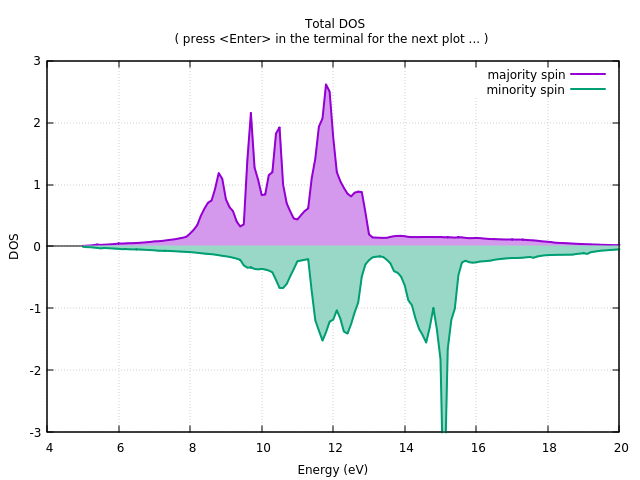
\includegraphics[scale = 0.5]{figs/D2/Fe_DOS.png}}
      \subfigure[]{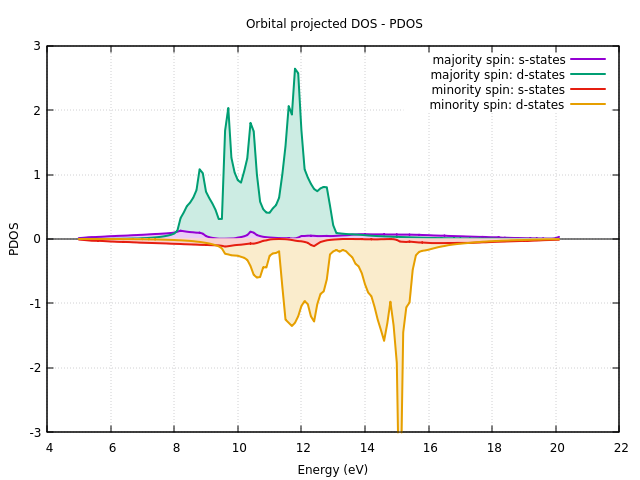
\includegraphics[scale = 0.5]{figs/D2/Fe_PDOS.png}}
      \caption{DOS y PDOS sobre los OA s y d para el Fe ferromagnetico. Majority y minority spin corresponden a spin up y down, respectivamente.}
  \end{figure}
